\chapter{Diagramme d'Acteurs}

\par Nous avons d�nombr� quatre acteurs logiques pour notre
application :
\begin{itemize}
\item {\bf Consultant :} Repr�sente n'importe qui pouvant acc�der �
l'intranet, un �tudiant par exemple. Il n'a pas de droits de
modification, il ne peut pas par exemple modifier un exercice. Il ne
poss�de aucun privil�ger except� la consultation de l'intranet et le
t�l�chargement de documents.
\item {\bf Enseignant :} Personne pouvant s'identifier sur
l'application. Elle pos�de des droits bien d�finis pouvant aller du
simple changement de mot de passe � la cr�tion d'un exercice. Cette
personne peut par exemple cr�er un exercice, lui ajouter une
correction, puis �ventuellemnt supprimer le tout.
\item {\bf Responsable :} Il repr�snte la personne pouvant cr�er/modifier un
enseignement. Cependant, par mesure de s�curit�, il n'a pas le droit
de supprimer un enseignement o� il est responsable. Cette personne
peut �tre repr�sent� par un enseignant. Il peut donner des droits sur
son enseignement.
\item {\bf Administrateur :} Personne qui g�re les comptes des
utilisateurs. Il peut en plus supprimer des enseignements.
\end{itemize}

\par Voici les d�pendances entre les differents acteurs :
\begin{center}
\scalebox{0.7}{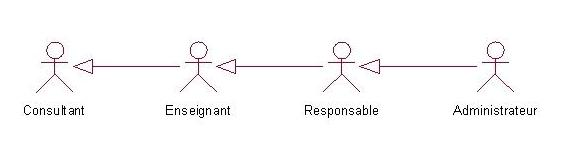
\includegraphics{images/Acteur.jpg}}\\
\par{Diagramme d'Acteurs}\\
\end{center}

\par Maintenant, voyons les differentes int�ractions entre l'application
Web et les acteurs.